\documentclass[12pt,a4paper]{article}
\usepackage{algorithm, algpseudocode, amsmath, amssymb, amsthm, bm, csquotes, emf, empheq, geometry, graphicx, hyperref, listings, mhchem, multirow, siunitx, caption, float, longtable}
\usepackage[italicdiff]{physics}
\usepackage[section]{placeins}
\usepackage[justification=centering]{caption}
\usepackage[column=O]{cellspace}
% \usepackage[extrafootnotefeatures]{xepersian}
\hypersetup{colorlinks=true, urlcolor=cyan}

\title{2D Ising model simulated with Metropolis algorithm}
\author{Zahra Akbari}
\date{}


% \settextfont{}
\linespread{1.2}

\setlength\cellspacetoplimit{5pt}
\setlength\cellspacebottomlimit{3pt}
\newcommand{\multlinecell}[1]{\begin{tabular}[c]{@{}c@{}}#1\end{tabular}}

\newcommand{\qfrac}[2]{\left(\frac{#1}{#2}\right)}
\newcommand{\fsqrt}[2]{\sqrt{\frac{#1}{#2}}}
\newcommand{\ddfrac}[2]{{\displaystyle\frac{\displaystyle #1}{\displaystyle #2}}}
\newcommand{\pdvc}[3]{\qfrac{\partial #1}{\partial #2}_{#3}}
\newcommand{\dbar}{{d\mkern-7mu\mathchar'26\mkern-2mu}}
\newcommand*{\defeq}{\mathrel{\vcenter{\baselineskip0.5ex \lineskiplimit0pt
			\hbox{\scriptsize.}\hbox{\scriptsize.}}}
	=}

\begin{document}
	\maketitle
	\section*{Theory and Methods}
	The Ising model
	consists of a 2D square lattice of spins that can be either up or down, and interact only with their nearest neighbors. The energy of a spin configuration is given by:
	\begin{align*}
	E(s) &= -J \sum_{i,j} s_i s_j - h \sum_{i} s_i	
	\end{align*}
	In this problem, Metropolis Mont Carlo algorithm is used to simulate the 2D Ising model. without any external magnetic field.
 the boundary condition is periodic.
The following quantities are calculated using the following formulas:

\begin{align*}
	E &= -\sum_{i,j} S_{i} S_j\\
	M &= \abs*{\sum_i s_i}\\
	C_v &= \frac{\beta^2 var(<E>)}{N^2}\\
	\chi &= \frac{\beta var(<M>)}{N^2}\\
\end{align*}
	where N is the grid size. $\beta$ is also considered 1 so that J is the variable in this problem.

	\pagebreak

	\section*{Results}
	The following results are obtained by simulating the 2d ising model with three grid sizes: 10,15,20.
	The function for implementing the metropolice algorithm is runned for 100000 time steps (using IsingMetroPolice function). At last Calculator function 
	is used to run the metropolice function for 100 runs, then the desired variables are obtained by meaning over the 100 results.
	At last we graph the variables over different Js:

			
			\begin{figure}[H]
				\centering
				\includegraphics[width=10cm]{cv.png}
				\caption{$C_v$ with 100000 metropolice time steps }
			\end{figure}

			\begin{figure}[H]
				\centering
				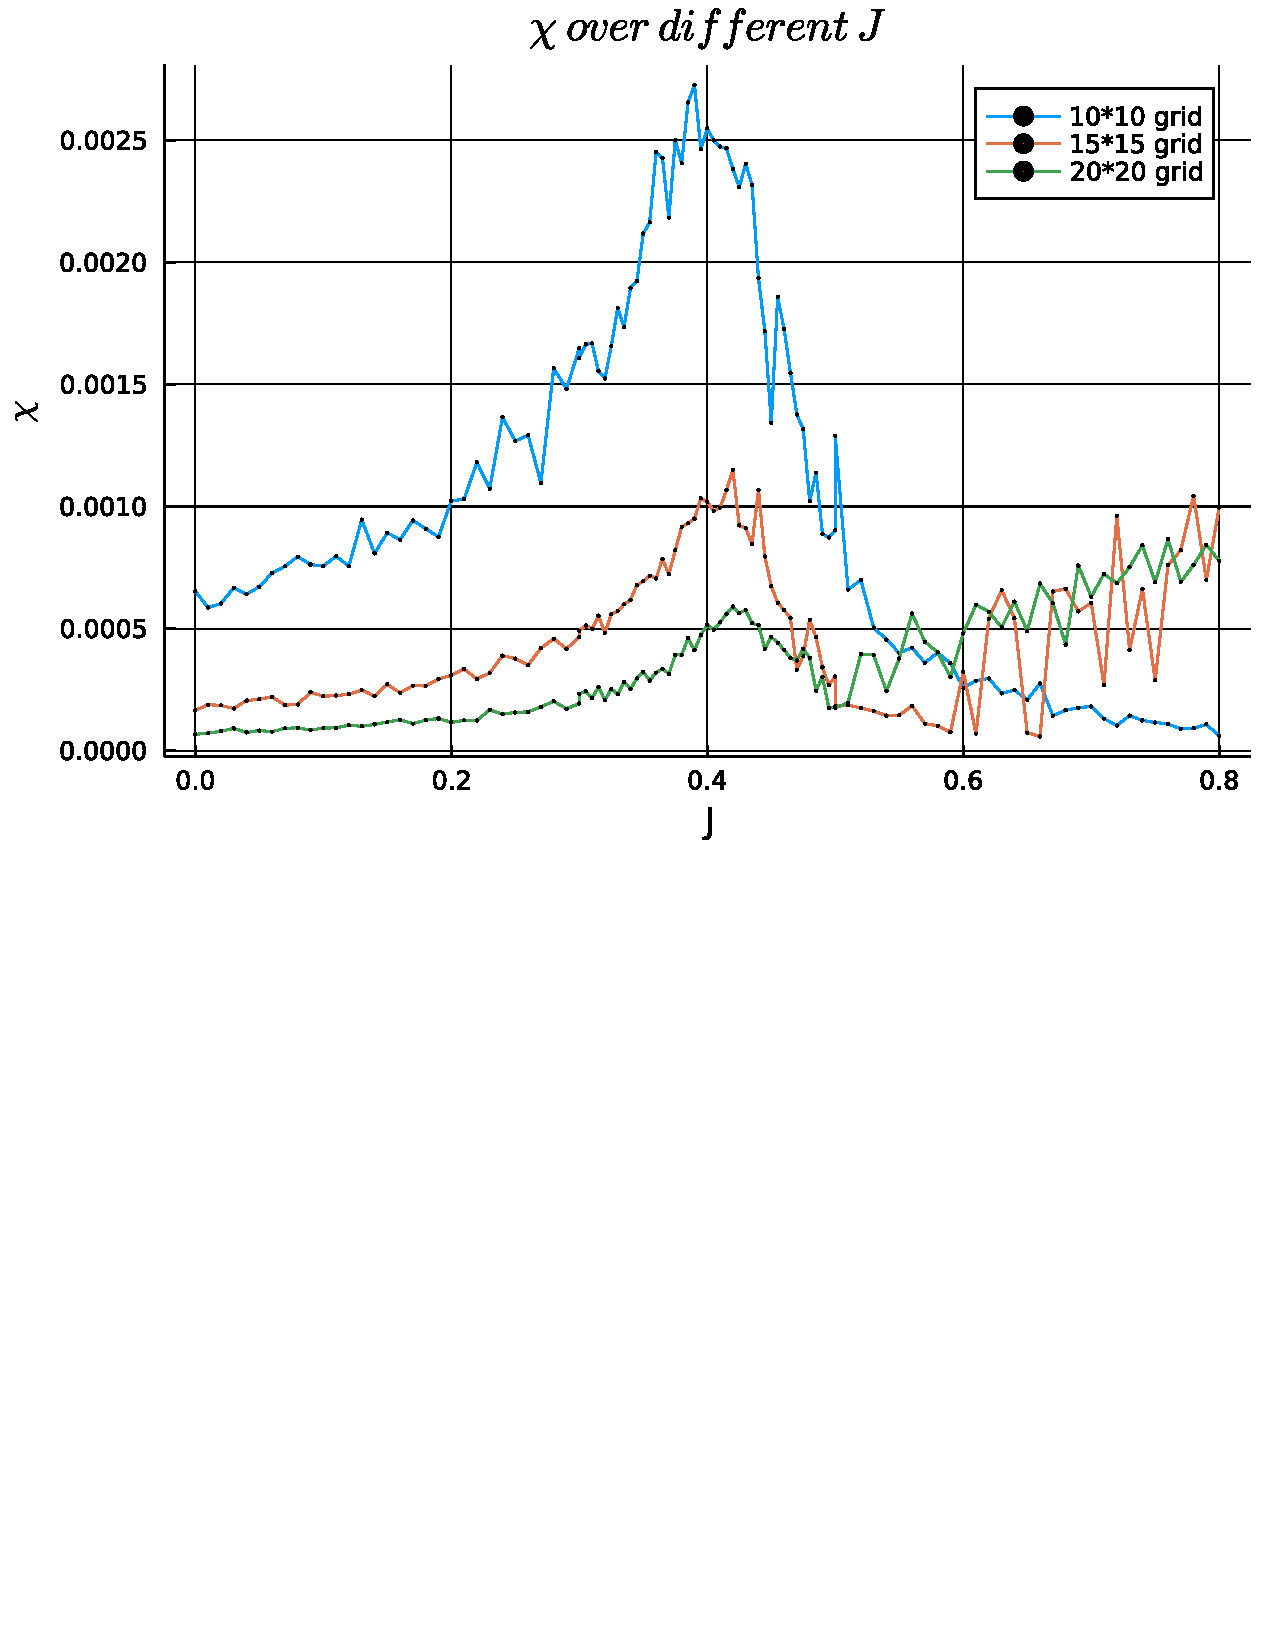
\includegraphics[width=10cm]{khi.png}
				\caption{$\chi$ with 100000 metropolice time steps}
			\end{figure}


			\begin{figure}[H]
				\centering
				\includegraphics[width=10cm]{m.png}
				\caption{$M$ with 100000 metropolice time steps}
			\end{figure}

			\begin{figure}[H]
				\centering
				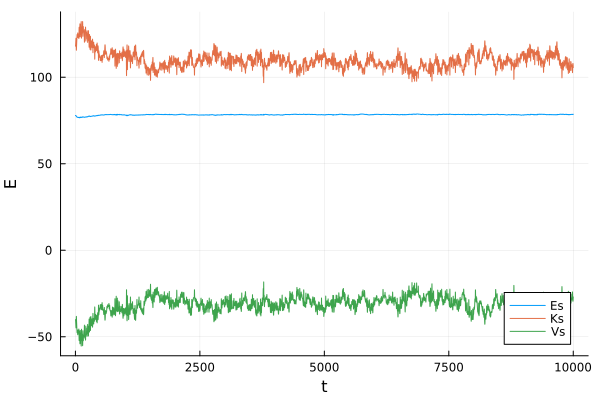
\includegraphics[width=10cm]{E.png}
				\caption{$E$ with 100000 metropolice time steps}
			\end{figure}
			For getting better results for finding the critical exponents, the used metropolice time step didn't seem sufficent. Thus the simulation was repeated for 20*20 grid with 1 million metropolice time steps.
			As this incresed the run time, multithreading was needed. Using @threads macro in julia the code took about 130 minutes to compile.

			\begin{figure}[H]
				\centering
				\includegraphics[width=10cm]{newcv20.png}
				\caption{$C_v$ with 1000000 metropolice time steps}
			\end{figure}

			\begin{figure}[H]
				\centering
				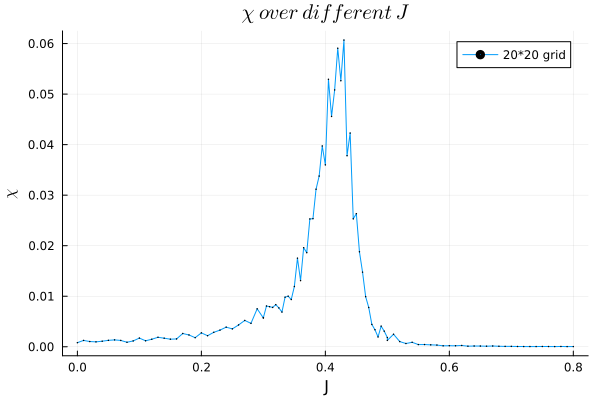
\includegraphics[width=10cm]{newkhi20.png}
				\caption{$\chi$  with 1000000 metropolice time steps}
			\end{figure}


			\begin{figure}[H]
				\centering
				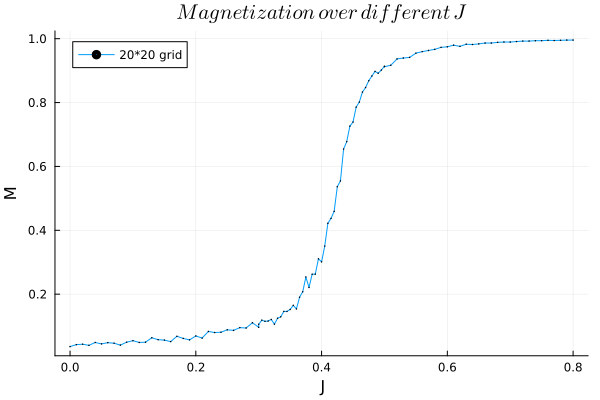
\includegraphics[width=10cm]{newM20.png}
				\caption{$M$  with 1000000 metropolice time steps}
			\end{figure}

			\begin{figure}[H]
				\centering
				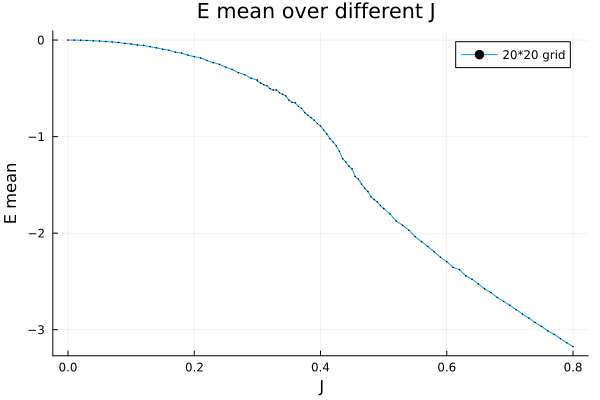
\includegraphics[width=10cm]{newE20.png}
				\caption{$E$  with 1000000 metropolice time steps}
			\end{figure}
			\pagebreak

			Testing the IsingMetroPolice functions with a sample 100*100 grid is illustrated below. 
			 the gif is also available.

			 \begin{figure}[H]
				\centering
				\includegraphics[width=10cm]{randgrid.png}
				\caption{Random grid generated}
			\end{figure}

			 \begin{figure}[H]
				\centering
				\includegraphics[width=10cm]{randgrid2.png}
				\caption{The grid after 50000 metropolice steps in T = 1}
			\end{figure}

			
\pagebreak
	\section{Statistics}		
 In another file (named data) the saved data is used for finding the critical exponents. We fit a line to logarithm of the variables over log(j) for finding the following exponents:

\begin{center}

	\begin{tabular}{|c|c|c|c|}
		\hline
	Relation & \multicolumn{2}{|c|}{Critical Exponent} & $T_c(\infty)$ \\
	\hline
	$C_V\sim c_0\ln{\abs{T-T_c}}$ & $c_0$ & -0.565 & 2.29 \\
	$\chi\sim\abs{T-T_c}^{-\gamma}$ & $\gamma$ & 2.05 & 2.35 \\
	$\expval{\abs{m}}\sim\abs{T-T_c}^{\beta}$ & $\beta$ &0.515 & - \\
	\hline
\end{tabular}
\end{center}

It should be noted that the line is fitted only to the critical interval just before the critical temperatre:

\begin{figure}[H]
	\centering
	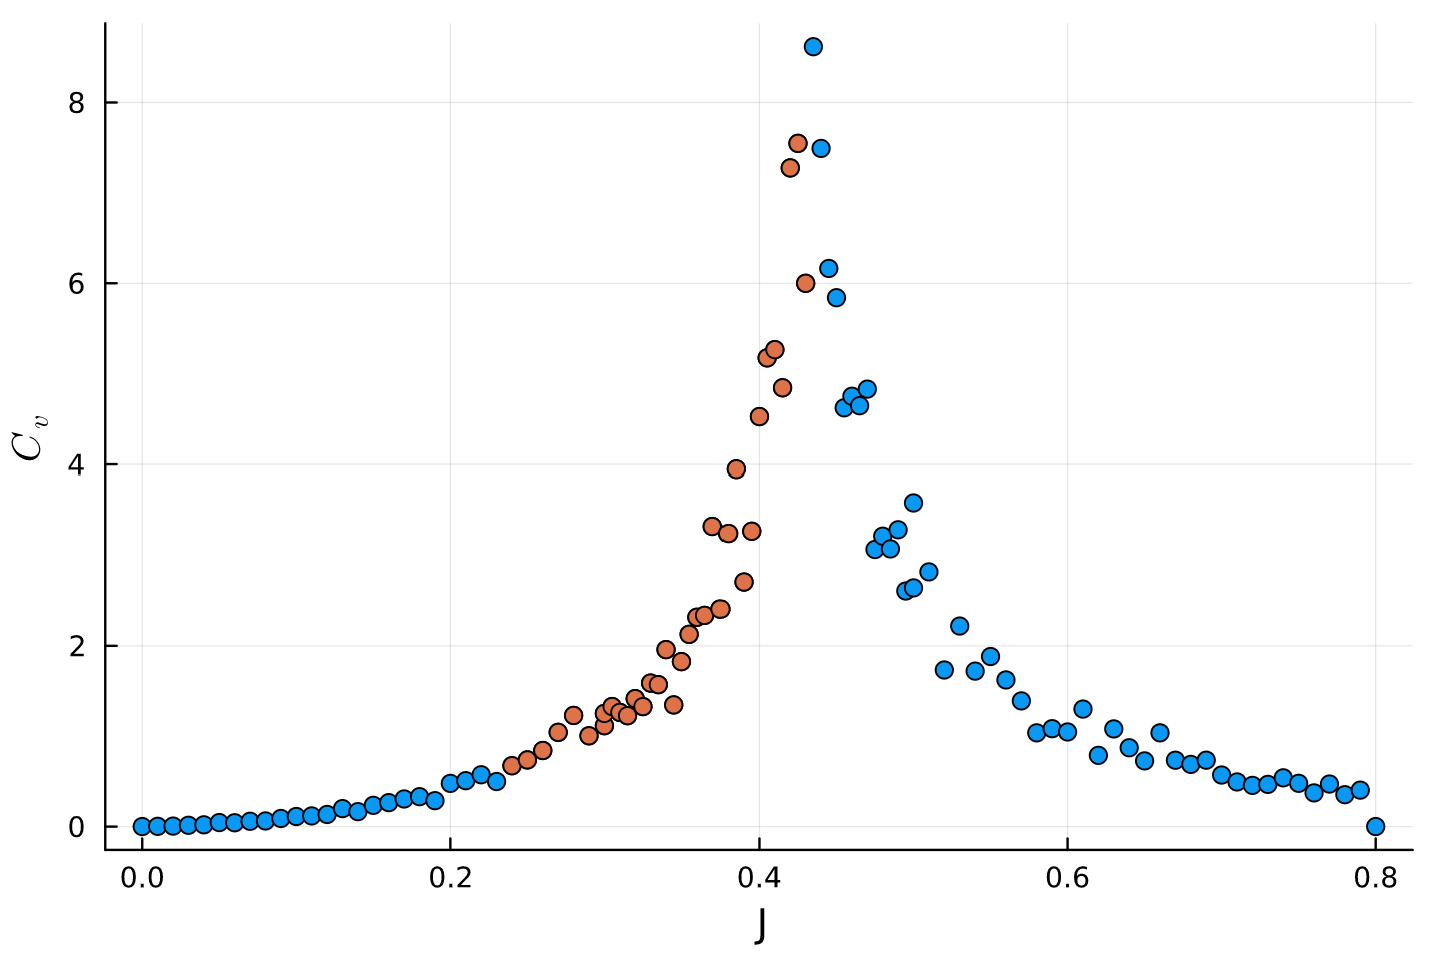
\includegraphics[width=10cm]{interval.png}
	\caption{The interval where critical exponents are extracted from. }
\end{figure}

\begin{figure}[H]
	\centering
	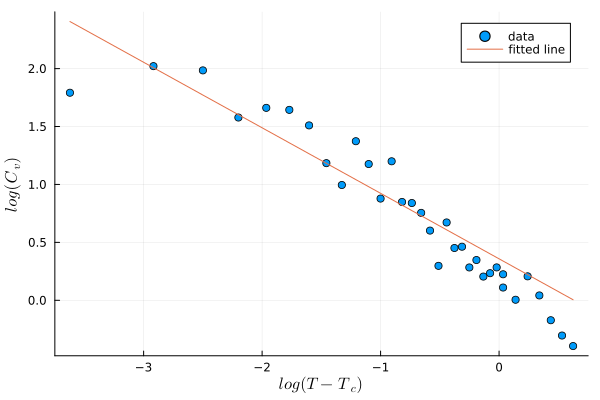
\includegraphics[width=10cm]{fitdata.png}
	\caption{An example: log(Cv) is fitted over $log(T-T_c)$ in critical interval for finding critical exponents. }
\end{figure}

An attemp was also made into finding critical exponents for correlation length. The following code is the method used. Though the resulting data doesn't seem working. The following graphs are AutoCorrelation for half of a grid:
\begin{figure}[H]
	\centering
	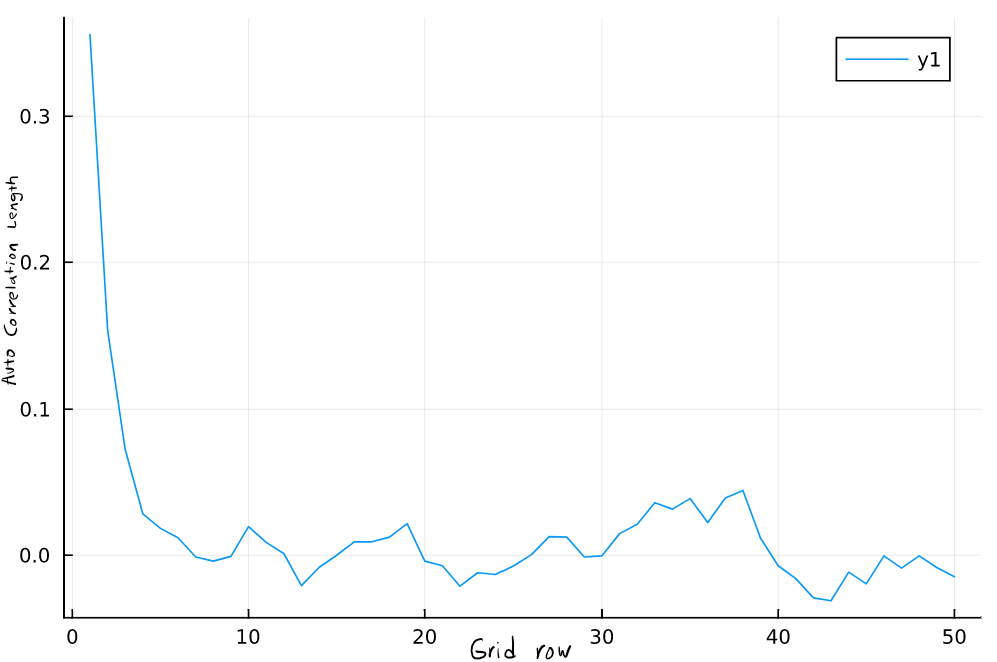
\includegraphics[width=10cm]{autoco100.png}
	\caption{Autocorrelation length going through half of a grid with 256 rows. }
\end{figure}
\begin{figure}[H]
	\centering
	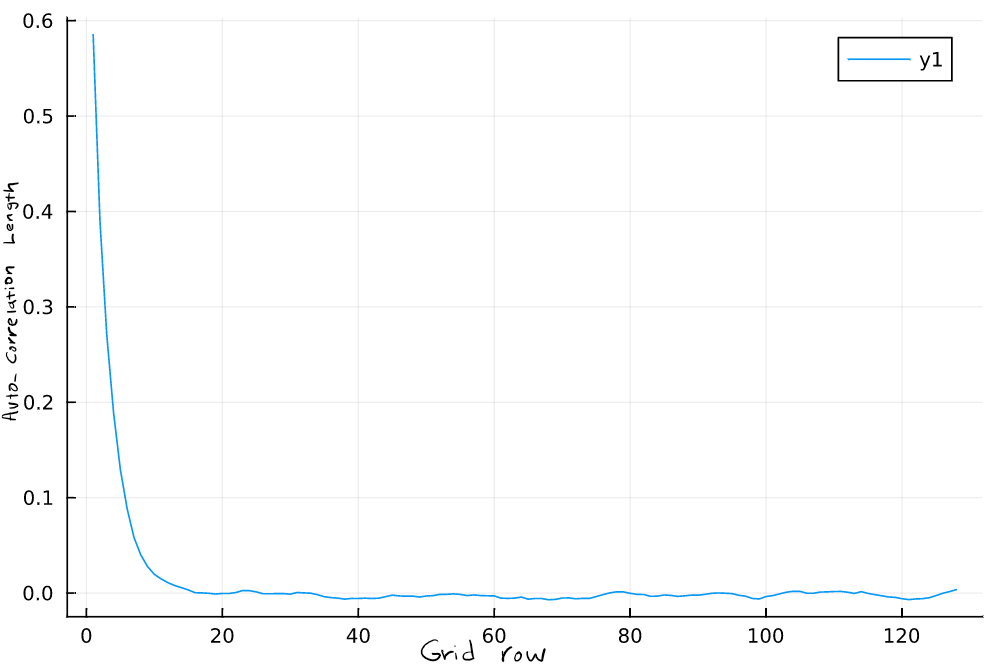
\includegraphics[width=10cm]{autoco256.png}
	\caption{Autocorrelation length going through half of a grid with 100 rows }
\end{figure}

\begin{figure}[H]
	\centering
	\includegraphics[width=10cm]{report.png}
	\caption{The code intended to calculate correlation length }
\end{figure}
			\end{document}
